\chapter{Evaluation}
\label{ch_evaluation}

This chapter explains the basics of working with PRISM model checker,
then describes how are the algorithms implemented as a part of PRISM,
how they behave on small models, and how do they compare to other
methods on standard models.

\section{PRISM, Probabilistic Model Checker}

PRISM \parencite{prism}
({\em probabilistic model checker}) is a program/framework
for formal modelling and analysis of probabilistic systems.
We show how to use PRISM to describe MDPs, their properties,
%and how to check them.

\subsection*{Describing MDPs with the PRISM language}
PRISM has a language for description of Markov decision processes
based on the formalism of Alur and Henzinger \parencite{ReactiveModules}.
A brief example is given below for the readers who wish to try our
algorithms on small models which they can describe and solve by hand.
The the definitive guide to the language is available online on the
PRISM homepage \parencite{prism_lang}.

The PRISM language describes {\em modules} (interacting actors),
their states (using variables) and transitions between the states.
An example single PRISM language line is below. The line translates as:
if condition \verb|guard| is satisfied the actor can choose action \verb|act|
and
with probability \verb|prob_1| update \verb|update_1| will happen,
with probability \verb|prob_2| update \verb|update_2| will happen,
and so on.

\begin{verbatim}
[act] guard -> prob_1 : update_1 + prob_2 : update_2 + ...
\end{verbatim}

\begin{figure}
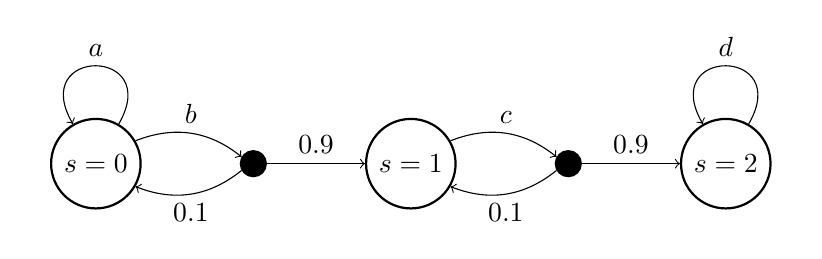
\begin{tikzpicture}
    \tikzstyle{state}=[thick,draw=black,circle]
    \tikzstyle{transition}=[draw,shape=circle,fill=black]
    \tikzstyle{loop}=[looseness=5, in=120, out=60]

    \node[state] at (0,0) (s0) {$s = 0$};
    \node[transition] at (2,0) (s0b) {};
    \node[state] at (4,0) (s1) {$s = 1$};
    \node[transition] at (6,0) (s1b) {};
    \node[state] at (8,0) (s2) {$s = 2$};

    \draw (s0) edge [loop,->] node [above] {$a$} (s0);

    \draw (s0) edge [bend left, ->] node [midway, above] {$b$} (s0b);
    \draw[->] (s0b) -- (s1) node [midway, above] {0.9};
    \draw (s0b) edge [bend left, ->] node [midway, below] {0.1} (s0);

    \draw (s1) edge [bend left, ->] node [midway, above] {$c$} (s1b);
    \draw[->] (s1b) -- (s2) node [midway, above] {0.9};
    \draw (s1b) edge [bend left, ->] node [midway, below] {0.1} (s1);

    \draw (s2) edge [loop,->] node [above] {$d$} (s2);
\end{tikzpicture}
\caption{Module M}
\label{moduleM}
\end{figure}

An example module is described below and is equivalent to the MDP
depicted in \autoref{moduleM}.

\smallskip
\begin{verbatim}
mdp // Tell PRISM this file describes an MDP
module M
    s : [0 .. 3] init 0;
    [a] s=0 -> (s'=0);
    [b] s=0 -> 0.9:(s'=1) + 0.1:(s'=0);
    [c] s=1 -> 0.9:(s'=2) + 0.1:(s'=1);
    [d] s=2 -> (s'=2);
endmodule
\end{verbatim}
\smallskip


A property we might be interested in is the maximum probability of
eventually reaching state \verb|s=2|, this could be described to PRISM
with the string \verb|Pmax=? [F s=2]|, where $F$ represents the
$\lozenge$ symbol used previously. A user can use standard logical
connectives for describing the target states. At the moment our
implementation does not support timed properties (i.e., \verb|F <= x| is not
supported), however, we expect it is not too hard to implement such
functionality.

\subsection*{Running PRISM}

We have a model description and a property but before we analyze it
PRISM has to be installed.
There is a modified version of PRISM distributed with this thesis. It
can be built by issuing the \verb|make| command inside the
\verb|prism/prism| directory. Java is a required prerequisite.
Once built the PRISM binary is available at \verb|prism/prism/bin/prism|.

Now use PRISM to analyze the model -- its name is passed as the first
argument and \verb|-pf| specifies the property we want to check.
The \verb|-ex| flag will be described later.
Running the command below
confirms our expectations: the maximum probability of eventually
reaching state \verb|s=2| is 1. If not specified otherwise, the
algorithm used is value iteration.

\medskip
\begin{verbatim}
./prism modelM.nm -pf 'Pmax=? [F s=2]' -ex
\end{verbatim}
\medskip

The following tells PRISM to use MCTS-BRTDP where the next state in
BRTDP is chosen to be the one with highest upper bound.

\medskip
\begin{verbatim}
./prism modelM.nm -pf 'Pmax=? [F s=2]' -heuristic_verbose \
 -heuristic MCTS_BRTDP -next_state HIGH_PROB
\end{verbatim}
\medskip

The UCB constant can be chosen with
\verb|-ucb1constant|. If not provided the value is set to
$1/\sqrt{2}$.

The heuristic method can be chosen out of the following:\linebreak
\verb|MCTS_BRTDP|, \verb|BRTDP|, \verb|BRTDP_UCB|. BMCTS is chosen by
using method \verb|MCTS_BRTDP| together with \verb|-next_action 5|.
The next state heuristics we use are
\verb|HIGH_PROB|, \verb|MAX_DIFF|.
The variation of BRTDP using UCB to select the next action is chosen by
adding \verb|-next_action 2|.

\subsection*{Data structures}
The \verb|-ex| switch used in the value iteration example above tells
PRISM to use the explicit computation engine.
The explicit computation engine explores the MDP and stores it in
a sparse matrix before the value iteration algorithm is run.
PRISM also offers three symbolic computation engines based on binary decision
diagrams.

All the heuristic methods use a data structure implemented in
\verb|prism/prism/src/heuristic/CachedModelGenerator.java|.
With this {\em model generator} data structure PRISM will not build the
whole MDP from its description unless asked to.
Asking the model generator to reveal parts of the model results in the
construction of an {\em explicit model} which is cached in the memory.
Such construction is computationally expensive and often unnecessary
which is when the heuristic methods perform so well.

\section{Implementation}

We describe how the pseudocode described in \autoref{ch_mcts} maps to
the implementation in PRISM. The implementation can be found in
\verb|prism/prism/src/heuristics| attached to the thesis.

To represent the MCTS tree we use classes \verb|MCTree.java| and
\linebreak
\verb|MCNode.java|. The tree class has method \verb|unfold|
which asks the model generator to add the next states of a given state
to the explicit model, and adds them to the tree.

The next state heuristics are implemented in a straightforward way
inside directory \verb|nextstate|. The tree heuristics described earlier
are implemented in directory \verb|treeheuristic|.

MCTS-BRTDP is implemented in \verb|search/MctsBrtdp.java|. The entry
point is \verb|computeProb|, subsequently
\verb|monteCarloTreeSearch| is invoked until the stopping condition
is reached (see method \verb|isDone|). Method
\verb|monteCarloTreeSearch| first selects and expands a tree state
(using \verb|treeSelectAndExpand|),
then uses \verb|exploreAndUpdate| implemented in BRTDP
(\verb|search/HeuristicBrtdp.java|) as the rollout and propagates
the values using updates to the root.

As we have observed problems only once during thousands of runs on our
models, we have not implemented the removal of subtrees induced by nodes
corresponding to a state which is contained in a collapsed MEC. The
increase in complexity of such implementation should not be significant.

BMCTS is implemented by modifying MCTS-BRTDP. The modification is turned
on when the flag \verb|next_action 5| is added to a command using
MCTS-BRTDP. This change makes the BRTDP implementation chose next action
uniformly at random instead of MAX-DIFF or HIGH-PROB.

\section{Behaviour on Small Models}

For small models, we used visualization to observe how MCTS-BRTDP solves
them. To render the progress of MCTS-BRTDP into a series of pictures,
the last lines of \verb|MctsBrtdp.monteCarloTreeSearch| have to be
uncommented.  Due to the randomized nature of the algorithms,
a researcher should observe more runs before making conclusions.

Three simple models are presented with a description of the methods'
approach to solving them.
The first is a model resembling a binary tree, second is
the BRTDP adversary, the third model offers a choice between a simple
path and a complex cloud. They can be found in directory
\verb|small_models| attached to the thesis.

\subsection*{Binary Tree Model}

The ``binary tree'' model features two decisions ({\em left} and {\em
right}) in each state and each decision has two successors,
the {\em left} one occurs with probability 0.2,
the {\em right} one with 0.8. A path through the model goes through 4 states
before it reaches a ``leaf'' state. Every leaf state of the subtree
induced by the left decision in root leads to state 85, every leaf state
of the other subtree leads to state 86. We ask what is the maximum
probability of reaching state 85.

By running the program repeatedly it can be observed that MCTS-BRTDP
almost evenly explores the branches in a balanced way while utilizing
BRTDP rollouts to search for promising paths. BRTDP on its own
selects a branch it knows the least about until it learns the upper bound
for the right part of the tree is 0 and therefore it has to focus on the
left part. The VCB for MCTS-BRTDP focuses on the left part quickly due
to successful results, however it still explores the right part a bit to
look for possibly missed target states and to decrease the upper bound.

\subsection*{BRTDP Adversary}

In \autoref{brtdp_adversary} MCTS-BRTDP has a clear advantage as it
traverses to a leaf of the tree and then adds a node to it with each iteration.
Soon the tree reaches the target state and it remains to perform updates
equivalent to value iteration.


\subsection*{Cloud And Path Model}

The model has an initial state,
``left part'', and ``right part''. Left part is a simple path to a
target state. Right part is comprised of states with randomly selected
choices and transitions but without a target state.
From the initial state there is an action to go left with probability
0.8 and right with probability 0.2, and another action with the same
effect but reversed probabilities.

MAX-DIFF BRTDP quickly learns that the upper bound in right part is
zero, abandons this part of the MDP to focus on the left part and learn
its upper and lower bound 0.8.

MCTS-BRTDP is forced to explore the right part too but learns the
correct value soon. On the other hand MCTS-BRTDP with the VCB formula
finds the target in the left part and then focuses too much on this part
even though what it needs is to learn that the right part has upper
bound 0 -- this variant is thus taking very long to find the correct
probability unless it is configured with a high multiplier in the
exploration term of the VCB formula.

Observing the VCB variant of MCTS-BRTDP on this and the binary tree
models suggests that it is quick to find good lower bounds. However,
then it commits to the good paths of the MDP so much that it has trouble
computing a better upper bound in the parts which do not lead to a
target way (as quickly as the exploited parts).

\section{PRISM Benchmark Suite and Other Models}

Experimental evaluation was done mainly on standard models
distributed with PRISM. Most of the MDPs described by these models are
concerned with network configuration where randomness plays important
role in achieving a common goal.
%We provide a brief, incomplete
%description of the {\em zeroconf} model to offer basic familiarity and
We
refer the reader to thorough descriptions of all the models on PRISM's
website.
%\href{http://www.prismmodelchecker.org/casestudies/}{www.prismmodelchecker.org/casestudies/}.

The description of the standard models in the PRISM language can be
found inside \verb|prism/tests/reachability/models| in the source codes
attached to this thesis. The properties checked are defined in
\verb|prism/tests/reachability/scripts/benchmark.py| for each model.

We also created new MDPs by combining the PRISM models with the MDP
which is hard for BRTDP (\autoref{brtdp_adversary}). We describe them in
the last subsection.

%\subsection*{Zero-configuration networking}

%{\em
%Zeroconf}\footnote{\href{http://www.prismmodelchecker.org/casestudies/zeroconf.php}{http://www.prismmodelchecker.org/casestudies/zeroconf.php}} model corresponds to a set of computers establishing a
%network without a given leader. Such leader could be a human setting
%static IP addresses or a DHCP server which would need to be configured
%up front -- in both cases there is extra work required.

%The zero-configuration networking protocol describes how should the
%computers proceed. Upon connecting to the network a computer picks an IP
%address at random and broadcasts its choice via an ARP packet called
%{\em probe} repeated $K$ times ($K=4$ by the standard) with two second
%delay. If another computer responds to one these
%ARP packets the original sender will then pick another IP address and
%repeat the process. If it does not receive a response it then broadcasts
%twice an ARP packet asserting this computer's use of the chosen IP
%address.

\subsection*{Combining PRISM models with BRTDP adversary}

We combined the MDPs in two ways. The first is by {\em branching} and the
resulting shape is shown in \autoref{fig:branching}.

\begin{figure}[h]
\begin{center}
\begin{tikzpicture}
    \tikzstyle{state}=[thick,draw=black,circle]
    \tikzstyle{transition}=[draw,shape=circle,fill=black]
    \tikzstyle{loop}=[looseness=5, in=120, out=60]

    \node[state] at (0,0) (s0) {0};
    \node[transition] at (1.6,0) (s0b) {};
    \node[state] at (3.2,0) (s1) {1};
    \node[transition] at (4.8,0) (s1b) {};
    \node[state] at (6.4,0) (s2) {2};
    \node[transition] at (8,0) (s2b) {};
    \node[state] at (9.6,0) (s3) {3};

    \node [cloud, draw,cloud puffs=10,cloud puff arc=120, aspect=2,
        inner ysep=1em] at (2,-3) (zconf) {zeroconf};

    \draw (s0) edge [bend right, ->] node [midway, right] {$b$} (zconf);

    \draw (s0) edge [bend left, ->] node [midway, above] {$a$} (s0b);
    \draw[->] (s0b) -- (s1) node [midway, above] {0.01};
    \draw (s0b) edge [bend left, ->] node [midway, above] {0.99} (s0);

    \draw (s1) edge [bend left, ->] node [midway, above] {} (s1b);
    \draw[->] (s1b) -- (s2) node [midway, above] {0.01};
    \draw (s1b) edge [bend left, ->] node [midway, above] {0.99} (s0);

    \draw (s2) edge [bend left, ->] node [midway, above] {} (s2b);
    \draw[->] (s2b) -- (s3) node [midway, above] {0.01};
    \draw (s2b) edge [bend left, ->] node [midway, above] {0.99} (s0);

    \draw (s3) edge [loop,->] node [above] {} (s3);

\end{tikzpicture}
\end{center}
    \caption{Combining zeroconf model with the BRTDP adversary in a
    branching manner.}
    \label{fig:branching}
\end{figure}

The second way to combine MDPs is parallel composition, which is done by
using modules in the PRISM language. Each state of the composed MDP is a member
of the product set of the sets of states of each of the modules. The
choice of the next transition is non-deterministic, i.e. a strategy does
not decide only which transition in a module to use but also which
module to use (the strategy for the MDP can be viewed as a member of the
product set of the set of strategies for each of the modules).

\section{Experimental Comparison}

On the following pages we present the results of our measurements.
In the presented tables rows correspond to models and their
configuration, columns to methods and chosen tree heuristic constant (in
parenthesis). Each table cell contains comma separated running time in
seconds and number of visited states of the MDP\footnote{The number of
states is, unlike running time, agnostic to implementation details.}\textsuperscript{,}\footnote{Value iteration has to construct the
whole model in memory but we show the number of states after VI
preprocessing.}. Hyphen denotes timeout or insufficient memory.

Each experiment shown in the tables below was repeated five
times and the results were averaged. There was no significant
variance in the measured times, so the number of repetitions is
sufficient and averaging provides representative results. We set
$\epsilon$ to $10^{-6}$.

We used a machine equipped with
40 cores of \verb|Intel(R) Xeon(R)| \verb|CPU E5-2630 v4 @ 2.20GHz| processors,
OpenJDK Runtime Environment 1.8 and JVM configured to use 4 GB of memory
and 512 MB stack size.

Our benchmark script which allows to describe each measurement
in an easy, declarative way is described in the appendix. See
\verb|prism/prism/tests/reachability/scripts/run_benchmark.py| for
\linebreak an example.
Results of many measurements, some of which were selected for the tables
presented later, can be found in directory \linebreak \verb|benchmarks| together
with a script for transforming them into a \LaTeX\ table.

In \autoref{table:general_comparison} we can see that MCTS-BRTDP-MAXDIFF can
keep up with BRTDP-MAXDIFF on the PRISM benchmark suite. Out of five
runs of BRTDP-UCB only one finished (in 35 seconds) in the time limit
(240 seconds). TODO: comment on the rest. BMCTS did not perform well on
any of the benchmarks.

\autoref{table:branch_zconf} shows how the methods perform on
branch-zeroconf. TODO: there should be one where mcts is better, one
when vi is better and one where brtdp is better, let's wait for the
results.
Note that overall the benchmarks MCTS-BRTDP does
not perform the worst or the best anywhere, making it a universal choice.

Measurements show that the only method which works on at least some of the
composition-zeroconf models is value iteration (specifically with $K = 40$ the
model has 141 thousand states and VI solves it, regardless of choice of $N$).
Other methods always run out of time.
But on composition-wlan6 we observed that MCTS-BRTDP is the only method which
can actually solve the problem. Moreover, it has to explore only few
thousands of states and a few seconds of running time.

The impact of tree heuristic constant is usually trivial and we did not
observe any cases where it would be beneficial to fine-tune the
constant. As it forces exploration, significant increases beyond a small
useful value just increased the number of explored states. This can be
seen in table TODO. (mcts-brtdp-md with ucb in 0.1,0.4,0.7,1,2,4,8,12,16
on firewire?)

\begin{landscape}

\begin{table}
\begin{tabularx}{\textwidth}{ l  | c | c | c | c }
                   & VI           &  BRTDP, MD       & MCTS-BRTDP-MD (0.5) & BRTDP-UCB (0.5)  \\
z-conf $N=15,  K=10$ & 205, 184k    &  0.93, 762       & 0.114, 819          &  12, 415         \\
z-conf $N=20,  K=10$ & 213, 184k    &  0.104, 769      & 0.110, 818          & 12.4, 436        \\
z-conf $N=20, K=20$  & -            &  0.129, 1172     & 0.172, 1208         & 12.7, 605        \\
z-conf $N=100, K=40$ & 16.2, 354k   &  0.27, 2191      & 0.268, 2375         & -                \\
firewire           &              &                  &                     & \\
wlan6              & -            &                  &                     & \\
coin               &              & -                &                     & \\
leader             &              &                  &                     &
\end{tabularx}
\caption{Comparison on standard PRISM models.}
\label{table:general_comparison}
\end{table}

\begin{table}
\begin{tabularx}{\textwidth}{ l  | c | c | c }
branch-zeroconf &    VI       & MCTS-BRTDP-MD (0.5) & BRTDP, MD  \\
$N=10,  K=10$     & 205, 1847k  &                     &            \\
$N=30,  K=10$     & 206, 1847k  &                     &            \\
$N=140, K=40$     & 16.5, 353k  &                     &
\end{tabularx}
\caption{Comparison on a ``branch'' model.}
\label{table:branch_zconf}
\end{table}

%\begin{table}
%\begin{tabularx}{\textwidth}{ l  | c | c
       %&  BRTDP, MAX-DIFF   &       VI     &  MCTS-BRTDP   & BRTDP-UCB \\
%wlan6  &             46,  &       204, &               & \\
%\end{tabularx}
%\caption{Composition models}
%\label{tab:composition}
%\end{table}
\end{landscape}

%\section{Model Structure and MCTS Performance}

%TODO: Explain why MCTS-BRTDP performs almost as well as BRTDP on some
%models

%We discuss what are the possible reasons MCTS performs well on some
%models and worse on others. (See e.g. On Adversarial Search Spaces and
%Sampling-Based Planning for a similar comparison between MCTS on Chess
%and Go).

%From the Chess and Go comparison it would seem that MCTS based methods would
%not perform well in verification as there are usually many dead ends.
%However by tuning the parameters and trying variants of the algorithms
%we have achieved better results on several models than other known methods.

%TODO :-/

%can we extrapolate where will each method do well from small instances of the models?
